% !TEX encoding = UTF-8 Unicode 
\documentclass[11pt]{article}
%\usepackage{CJKutf8}
\usepackage[english]{babel}
\usepackage{acl2014}
\usepackage{times}
\usepackage{url}
\usepackage{amsmath}
\usepackage{amsfonts}
\usepackage{amssymb}
%\usepackage{algorithmic}
\usepackage{enumerate}
\usepackage{latexsym}
\usepackage{graphicx}
\usepackage{verbatim}
\usepackage{chngpage}

% New commands serve as shorthand for frequently used command combinations.
\newcommand{\ind}[1]{\mathbf{1}\left(#1\right)}
\newcommand{\bx}{\mathbf{x}}
\newcommand{\by}{\mathbf{y}}
\newcommand{\bu}{\mathbf{u}}
\newcommand{\bw}{\mathbf{w}}
\newcommand{\br}{\mathbf{r}}
\newcommand{\E}{\mathbf{E}}
\newcommand{\D}{\mathbf{D}}
\newcommand{\R}{\mathbf{R}}
\newcommand{\bP}{\mathbf{P}}
\newcommand{\X}{\mathbf{X}}
\newcommand{\N}{\mathcal{N}}
\newcommand{\mH}{\mathcal{H}}
\newcommand{\argmin}{\operatornamewithlimits{argmin}}
\newcommand{\argmax}{\operatornamewithlimits{argmax}}

%%AL-COMMENTS insert title and name here
\title{Predicting Translation Difficulty on Sentence-level for MT Systems}

\author{
	Junyi Jessy Li and Kai Hong\\
   University of Pennsylvania \\
   Philadelphia, PA 19104 \\
  	{\tt \{ljunyi, hongkai1\}@seas.upenn.edu}}

\begin{document}
\maketitle

\section{Introduction}

Machine Translation (MT), despite its many recent advances, still remains a hard problem. 
Translations produced by automatic systems suffer from problems such as information reordering, misalignments, mistranslations, etc. 
In this study, we propose to explore the question of how difficult a sentence is to translate automatically. 

Intuitivelly, some sentences are easier to translate, while the others are much more difficult.
Consider the following quote: {\em ``Time flies like an arrow; fruit flies like a banana."}
The first half of the sentence means that time passes very quickly just as an arrow; while the second half of the sentence means that a ``fruit fly" enjoys eating a banana.
These kind of sentences could bring big problems for not only human, but also for MT systems. 
Thus, we propose that some factors might make the sentences difficult to translate, independent of language. Length, for instance, is a natural indicator for how difficult for a human to translate a sentence \cite{mishra-bhattacharyya-carl:2013:Short}. We ask the question whether it is also the case for automatic systems. Other indicators we conjecture include the use of subordinations, structure, amount of re-ordering and complexities of verb phrases and noun phrases, etc.

A handful of studies have looked into predicting the difficulty of translation on language level, rather than on sentence level. There, most of the work investigate the general properties which make those language-pairs difficult to translate. \newcite{birch-osborne-koehn:2008:EMNLP} show that the amount of reordering, morphological complexity and historical relatedness are important factors for predicting the performance of MT systems. A further study looked into 462 language pairs (in total 22 languages), where the concept of translation model entropy is introduced to capture the amount of uncertainty involved in choosing candidate translation phrases \cite{sys462}.

Through this study we hope to characterize difficulties that may lie ahead for MT systems, and we aim at quantitatively estimate such difficulties by developing a set of features for a machine learning framework.

\section{Datasets}
We collect our data from the test set of WMT 2011 \cite{callisonburch-EtAl:2011:WMT}, WMT 2012 \cite{callisonburch-EtAl:2012:WMT} and WMT 2013 \cite{bojar-EtAl:2013:WMT}.
The data from these three years include language pairs of English-German, English-French, English-Spanish and English-Czech in both directions. 
Thus a number of language families have been covered, including Germanic (English and German), Romance (French and Spanish) and Slavic (Czech) languages.
For each year, there are about 3,000 segments in all of the languages. 
We use the data of WMT 2012 and WMT 2013 for training. 
The data from year 2011 is split into development set and test set.
We use the first 1500 segments for each language pairs as test set, the other 1503 segments as develpment set. 
The data is available here:\\
\begin{footnotesize}{\tt /project/cis/nlp/data/corpora/wmt\_test/}\end{footnotesize}
We employ the average of BLEU scores produced by various MT systems as our main indicator of translation difficulty. Detailed objection function and evaluation is introduced in the next section.

\section{Objective Function and Evaluation}
We aim to collect a set of factors of a sentence that are indicative of translation difficulty. 
One challenge of such an approach is the lack of a reliable sentence-level evaluation metric for translation hypothesis. 
We conjecture that with more systems, the average of automatic scores would provide a partial but feasible solution to this problem.
Here, we regard BLEU scores as our goal of prediction. 
We directly use the code of smoothed BLEU which has been provided in Homework 4  (\texttt{bleu.py}) \cite{Liang:2006:EDA:1220175.1220271}.
The {\bf oracle translation difficulty} for a sentence is thus the average of BLEU scores of all MT systems, where higher score indicates easier sentence-pairs.
For example, consider we want to translate a sentence $e_1$ from English into French. 
We have 3 MT systems which translate the sentence $e_1$ into $f_1$, $f_2$ and $f_3$. 
Suppose the BLEU score of the sentences $f_1$, $f_2$ and $f_3$  are respectively 0.1, 0.2 and 0.15; 
Then the {\bf sentence difficulty} for sentence $e_1$ is 0.15.
Suppose we have another sentence $e_2$ with an average BLEU score of 0.5, then the sentence $e_2$ is easier than sentence $e_1$ due to its higher BLEU scores.
The average of BLEU scores have been used in similar ways by \newcite{birch-osborne-koehn:2008:EMNLP} and \newcite{sys462} where they evaluate langauge-level difficulty; 
as well as \newcite{nenkova-louis:2008:ACLMain} where they average over the ROUGE scores to predict input difficulty for automatic summarization.

To make our computation of the difficulty scores more credible, we only use the systems which are implemented on all 4 language pairs (FR-EN, ES-EN, CZ-EN, GR-EN). 
There are 13 systems satisfying this standard for WMT 2013, 5 systems for WMT 2012 and 4 systems for WMT 2011.

For this project, we only look into the difficulty translating from English to the other languages. 
This makes it easy for us to do deeper linguistic analysis. 

We propose two measures of evaluations as objective functions. 
Our main metric is \textbf{Pairwise Accuracy}. We answer the question that whether a sentence A is more difficult than a sentence B. 
We compute the ratio of correctly answering this question, which ranges between 0 and 1. Higher score indicates better prediction.
We take the average over the accuracy of all four language pairs as our \textbf{single final score}.
This is the main objective function we aim at optimizing. 
Apart from that,  we also compute the \textbf{Spearman Correlation} between the scores assigned to the sentences and the oracle scores.
This value ranges between -1 and 1. Still we take the average of Spearman Correlation across our four langauge pairs. 

\section{Default System}
\label{ssec:default}
Intuitively, one would feel longer sentences more difficult to translate. 
Such an effect was shown in humans in \newcite{mishra-bhattacharyya-carl:2013:Short}.
Therefore, we use the sentence length of source (English) sentence as our default system. 
We observe the \textbf{surpring} (yet doubtful) fact that longer sentences are actually having higher BLEU scores.
That said, longer sentences are easier to translate for MT systems.
The pairwise accuracy and correlation are both high using this feature, as shown in Table \ref{basictable}.
We here show a scatter plot of sentence length vs average BLEU scores in Figure \ref{fig:aa}, evaluated on EN-DE translation for WMT-12.
The Spearman Correlation of this case is 0.3342. 
According to the graph, we can see that long sentences seldomly gets too low or too high BLEU scores, in contrast to short sentences whose BLEU scores varied a lot. 

\begin{figure}[htbp]
\small
\centering
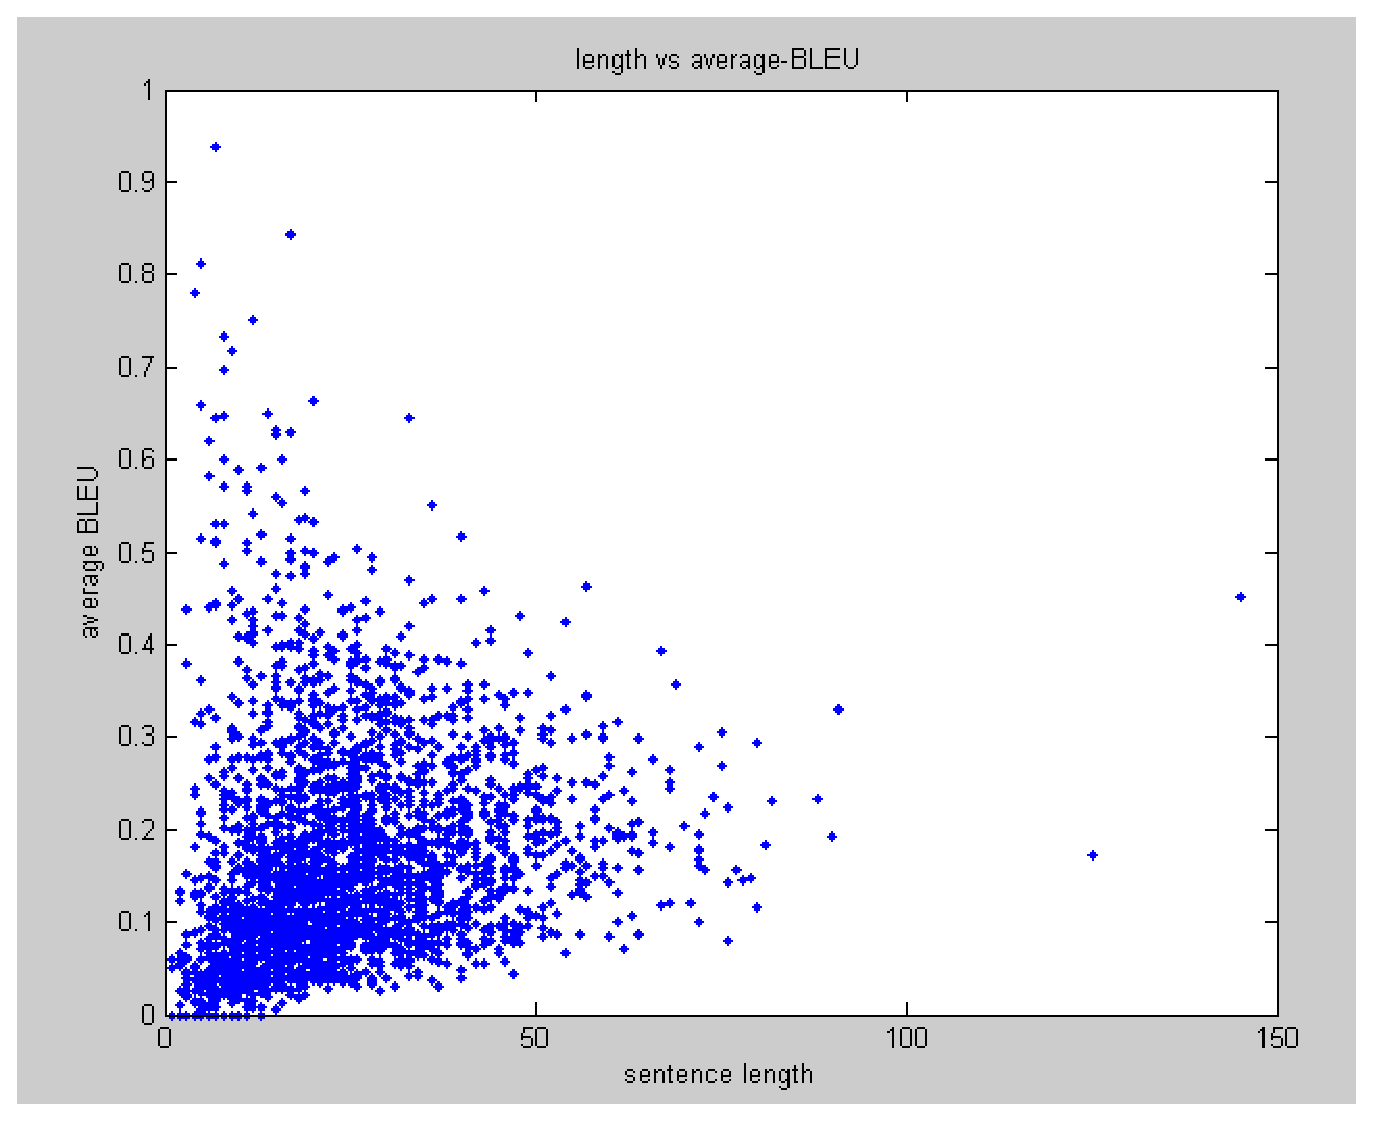
\includegraphics[height=65mm]{length_spearman.eps}
\caption{Sentence length vs average BLEU scores on WMT-12}
\label{fig:aa}
\end{figure}


\section{Baseline System}
We implement a system using the number of senses for the most polysemous word in sentence. 
We derive this score by counting the number of synsets for the words in sentence using Wordnet \cite{Miller95wordnet:a}. 
%This feature has also been discussed in prior work Table \ref{basictable}, however they take the average number of senses for word in the sentence. 
Again we observe the surprsing phenomenon that the setences with the most polysemous words are the ones with higher BLEU scores (See Table \ref{basictable}). 
This might be a side-effect that longer sentences actually have more polysemous words than shorter sentences. 
Note here that the baseline system does not give as good performance as the default system. 

\begin{table}[ht]
\centering
\begin{small}
\begin{tabular}{c|cc|cc}
& \multicolumn{2}{c|}{Dev set} & \multicolumn{2}{c}{Test set} \\ \hline
Feature & PAcc & Corr & PAcc & Corr \\ \hline \hline
Default  & 0.5993 & 0.2948 & 0.6189 & 0.3442 \\
Baseline & 0.5373 & 0.1185 & 0.5375 & 0.1060 \\
POS-unigram & 0.6008 & 0.2964 & 0.6115 & 0.3286 \\
Reg-All & 0.5465 & 0.1030 & 0.5589 & 0.1334 \\
Reg-Selected & 0.5795 &  0.2367 & 0.5849 & 0.2515 \\
\end{tabular}
\end{small}
\caption{Pairwise accuracy (PAcc) and correlation coefficient (Corr) for five selected systems, averaged across all languages.}
\label{basictable}
\end{table}

\section{Features}
Next we analyze a number of features and their discriminative powers for this task.
We develop four classes of features: surface features, syntax features, part-of-speech (POS) features and language model features. 
We first employ these features alone, as we do for default and baseline systems.
We later combine the features using Support Vector Regression in Liblinear \cite{Fan:2008:LLL:1390681.1442794}. 

\subsection{Surface Featurs}
\paragraph{Sentence length} As described in Section \ref{ssec:default}.
\paragraph{Punctuation marks} The number of punctuation marks in the sentence. If a sentence is divided into multiple segments, we hypothesis that the structures could be easier in each segment.

\subsection{Syntax Features}
Intuitively the complexity of an English sentence may contribute to how difficult it is to translate. \newcite{Chae:2009:PFT:1609067.1609082} studied the role of syntactic structures in accessing text fluency, including the fluency of sentences produced by MT systems. Here we present a series of syntactic factors computed on the {\em source} sentence. Here we use the Stanford Parser \cite{Klein03fastexact}. 

\paragraph{Depth of the parse tree} The maximum depth of the parse tree for each sentence. This feature is also highly related to the length of sentence.
\paragraph{Subordination} The total number of words involved in a subordination clause, normalized by the sentence length. In addition to the count of {\em wh}-words, the complexity of the clauses themselves might be indicative.
\paragraph{Phrase lengths} Here we compute: 1. the average length of all PP, NP, VP, ADJP, ADVPs in the sentence; 2. The maximum length of NP, VP, PPs in the sentence. Phrase lengths may impact language model probabilities and the use of phrase tables. Such features were also used in \cite{Chae:2009:PFT:1609067.1609082}.
\paragraph{Word specificity} For each noun, verb, adjective and adverbs in the sentence, we look up its specificity in WordNet by calculating the maximum path length to the root in the WordNet hierarchy.
\paragraph{Production rules} All production rules appearing in the syntactic parse tree of the sentence. Production rules are a node plus all its children, and supposedly should also capture the structural complexity of a sentence.
\paragraph{Number of {\em wh}-words} We count the number of {\em wh}-determiners, {\em wh}-pronouns and {\em wh}-adverbs in the sentence. {\em wh}-words are a good indicator of clauses in the sentence.

\subsection{Part-of-speech Features}
\paragraph{Part-of-speech} Here we use uni-, bi-, tri-, and four-grams of part-of-speech tags in the sentence. These features might also be indicative of how normal or unusual one sentence is.
\paragraph{Function words} We compute the fraction of function words (marked by their part-of-speech tags) in the sentence.

\subsection{Language Model Features}
We employ language model (LM) for predicting the whether a sentence is difficult or not.
A difficult sentence should be the ones which include rare words, phrases and the ones which are less fluent.
In statistical MT, the LM for the target language is an essential component during the decoding process. 
In our project, we trained our LMs from 160K documents in the New York Times corpus \cite{nytcorpus} using SRILM \cite{SRILM}. 
When a new English sentence comes, we compute its perplexity using the LM we trained. 
We experiment with unigram, bigram and trigram language models. 

\section{Results}
We study the impact of the features we proposed. 
For real valued features, we directly use  the feature values to calculate the pairwise accuracy and correlation coefficient (See Table ~\ref{tab:indivresults1}). 
For categorical features, we use Support Vector Regression available in the {\em LIBLINEAR} package \cite{Fan:2008:LLL:1390681.1442794} to learn a regression model, and then calculate the pairwise accuracies and correlation coefficient likewise. 
We show the two values for categorical features (part-of-speech N-grams and production rules) in Table~\ref{tab:indivresults2}.
Finally, we train two regression models including all features or some of the highly discriminative features.
The results are shown in Table ~\ref{basictable}.

Most of the features listed, except for the number of {\em wh}-words and average specificity, are significantly correlated with average BLEU scores. 
In fact, it can be seen in Table ~\ref{tab:indivresults1} that sentence length is the best feature.
However, we argue that one should caution against this conclusion; it could be possible that, since BLEU is precision based, and includes a length factor, that sentence length is significantly related with BLEU score
in itself.  
The BLEU version we are using (BLEU 4-gram with smoothing) also seems to suggest long sentences should have higher scores, 
since there is more room to hit a 4-gram when sentence becomes longer, and there is more room to improve the BLEU score for longer sentences by making the sentences shorter. 
The number of punctuations and depth of the parse tree are also highly correlated with sentence length. On the other hand, punctuations may confirm our conjecture that sentence structure decompose into segments that are simpler to translate. The length of phrases are also positively correlated with average BLEU scores. 
%One might link such correlation with higher probabilities given by the language model, and entires in the phrase table. Interestingly, average word specificity, even though not significant, are negatively correlated with average BLEU score. Specific words usually provide much detail and specific sentences may have less entries in a corpus, thus harder to model.

The language model perplexity correlates negatively with the sentence difficulty, as shown in Table \ref{tab:indivresults1}.
This is intuitive, since low perlexity indicates high probability, and that high probability positively correlates with higher average BLEU scores.
Interestingly, as the order of N-grams goes up, the indicabiality of LM features goes up. 
This might indicate that the fluency or difficulty of sentences might be better detected with larger n-grams being used. 

\begin{table}[ht]
\centering
\begin{small}
\begin{tabular}{c|cc|cc}
& \multicolumn{2}{c|}{Dev set} & \multicolumn{2}{c}{Test set} \\ \hline
Feature & PAcc & Corr & PAcc & Corr \\ \hline \hline
{\bf length} & 0.5993 & 0.2948 & 0.6189 & 0.3442 \\
treedepth & 0.5735 & 0.298 & 0.5887 & 0.2492\\
\# punctuations & 0.5454 & 0.1735 & 0.5758 & 0.1928 \\
wh-words & 0.4962 & 0.0897 & 0.5599 & 0.0974 \\
len-sbar & 0.5328 & 0.1216 & 0.5637 & 0.1521 \\
{\bf avglen-phrase} & 0.5734 & 0.2176 & 0.5894 & 0.2659 \\
{\bf maxlen-VP} & 0.5841 & 0.2524 & 0.5954 & 0.2766 \\
maxlen-NP & 0.5779 & 0.2396 & 0.6039 & 0.2984 \\
maxlen-PP & 0.5738 & 0.2289 & 0.5978 & 0.2787 \\
frac-func & 0.5524 & 0.1566 & 0.5542 & 0.1568 \\
avgspecificity & 05152 & 0.0458 & 0.5285 & 0.0833 \\
LM-uni perplexity & 0.5311 & -0.091 & 0.5126 & -0.0626 \\
LM-bi perplexity& 0.5221 & -0.0636 & 0.5062 & -0.0175 \\
LM-tri perplexity & 0.5533 & -0.1557 & 0.5335 & -0.0979 \\
\end{tabular}
\end{small}
\caption{Pairwise accuracy (PAcc) and correlation coefficient (Corr) for each real-valued features, averaged across all languages.}
\label{tab:indivresults1}
\end{table}

Both part-of-speech features and production rules are highly indicative of average BLEU score. 
As the order of N-grams goes up (up to trigrams), the indicability of such features go down. 
On the other hand, note that four-grams are actually better than tri-grams. One possible reason could be that the feature space explodes with higher order N-grams; but sentence structure is more and more captured with higher order N-grams. We leave this investigation to future work.

\begin{table}[ht]
\centering
\begin{small}
\begin{tabular}{c|cc|cc}
& \multicolumn{2}{c|}{Dev set} & \multicolumn{2}{c}{Test set} \\ \hline
Feature & PAcc & Corr & PAcc & Corr \\ \hline \hline
POS-uni & 0.6008 & 0.2964 & 0.6115 & 0.3286 \\
POS-bi & 0.5832 & 0.2477 & 0.5880 & 0.2612 \\
POS-tri & 0.5711 & 0.2116 & 0.5643 & 0.1920 \\
POS-four & 0.5845 & 0.2498 & 0.5721 & 0.2158 \\
Prodrules & 0.5717 & 0.2132 & 0.5658 & 0.1973 \\
\end{tabular}
\end{small}
\caption{Pairwise accuracy (PAcc) and correlation coefficient (Corr) for each categorical features, averaged across all languages.}
\label{tab:indivresults2}
\end{table}

We finally experiment with a full-blown regerssion system for prediction.
Using all of the features introduced, our model achieves a pairwise accuracy  of $54.7\%$ on developments set,  an accuracy of $55.9\%$ on test set.
The discriminative power of this system is not as good as some of the single features.
Secondly, we select the features which gives performance better than $57\%$ on development set. 
Then we use those features to train a classifier, which gives an accuracy of $58.0\%$ on training, $58.5\%$ on testing.
Our full-blown regression system does not succeed in beating the default system using sentence length.

\section{Conclusion}
We investigate the problem of predicting translation difficulty for MT systems.
We disclose the surprising fact that the average  BLEU score correlates positively with sentence length.
We propose a number of syntax features, POS-features and LM-features, while most of them show discriminative power compared with random.
However, none of the features give better pairwise accuracy compared with sentence length.
For future study, we propose to use human evaluations of fluency, adequency or HTER as a better oracle of translation difficulty.

\bibliographystyle{acl}
\bibliography{references}
\end{document}